\chapter{Lipkin-Meshkov-Glick model}
\label{chap:lipkin}

The Lipkin-Meshkov-Glick (LMG) model is a simple model manifesting the quantum phase transitions. It was introduced as a toy model for many-body fermion systems, but its applications are much wider. Generally it describes any \emph{fully connected qubit system}. \emph{Fully connected} means the interactions have infinite range. In the \emph {qubit system}, the individual atoms have only two energy eigenstates. This chapter aims to understand the properties of the ground state and its influence on different driving protocols. Understanding the fidelity during the phase transitions is important, because these changes are often present in the quantum annealing.

\section{Hamiltonian}
The LMG model is defined on a parametric space $\llambda\equiv (\lambda;\chi)\in\mathcal U\coloneqq \R^2$ with Hamiltonian
\begin{equation}
    \HH(\lambda,\chi)=\J_3+\lambda\hat V_1 +\chi \hat V_2+\chi^2 \hat V_3,
    \label{eq:firstOrderTransitionHamiltonian}
\end{equation}
where
\begin{align}
    \hat V_1 &\coloneqq-\frac{1}{2j}\J_1^2\\
    \hat V_2 &\coloneqq -\frac{1}{2j}\left[\J_1(\J_3+j\Id)+(\J_3+j\Id)\J_1\right]\\
    \hat V_3 &\coloneqq -\frac{1}{2j}(\J_3+j\Id)^2,
\end{align}
and \emph{angular momentum operator} $\bm\J=(\J_1,\J_2,\J_3)^T$.

Using the Spherical harmonics\footnote{https://mathworld.wolfram.com/SphericalHarmonic.html} basis $\{\ket{j,m}\}$ for quantum numbers $j$ as the angular momentum and $m$ its projection to the direction of $\J_3$ and defining
\begin{equation}
    \J_\pm\coloneqq\frac{1}{2}(\J_1\pm i\J_2),
\end{equation}
we get matrix elements
\begin{align}
    \braket{j'm'|\J^2|jm} &= j(j+1)\delta_{j'j}\delta_{m'm}\\
    \braket{j'm'|\J_3|jm} &= m \delta_{j'j}\delta_{m'm}\\
    \braket{j'm'|\J_\pm|jm} &= \sqrt{(j\mp m)(j\pm m+1)}\delta_{j'j}\delta_{m'm\pm 1},
\end{align}
where $\delta_{a'b}$ is Kronecker delta. The Hamiltonian can then be written as
\begin{equation}
\begin{split}
        % \left(\J_1+\chi(\J_3+j)\right)^2 &= \textcolor{purple}{\J_1^2} +\chi^2 (\J_3^2+j^2\Id+2j\J_3)+\chi(\textcolor{blue}{\J_1}\J_3+\J_3\textcolor{blue}{\J_1})+2\chi j\textcolor{blue}{\J_1}\\
        % \textcolor{purple}{\J_1^2}&= \frac{1}{4}(\J_++\J_-)^2= \frac{1}{4}(\J_+^2+\J_-^2+\textcolor{violet}{\J_+\J_-}+\textcolor{violet}{\J_-\J_+})\\ 
        % \textcolor{violet}{\J_\pm\J_\mp}&=\J^2-\J_3^2 \mp \J_3\\
        % \textcolor{blue}{\J_1}&=(\J_+ +\J_-),\\
        \HH =& J_3-\frac{\lambda}{8j}(J_++J_-)^2-\frac{\chi}{4j}\left[(J_++J_-)(J_3+j\Id)+(J_3+j\Id)(J_++J_-)\right]\\
        &-\frac{\chi^2}{2j}(J_3+j\Id)^2,
\end{split}
\end{equation}
which has penta-diagonal matrix representation. During the whole chapter, $j=N/2$ is used. 

First, the low dimensional cases of the Hamiltonian are analyzed, especially $N=3$, where the analytical formula for energy spectrum can be found. The limit $N\rightarrow \infty$ is then taken, showing the correspondence to the classical system. Finally, some generalization to an arbitrary dimension and an example of transport using quenches is presented. 











\section{Geometry for fixed dimension}
Because of a penta-diagonal form of the Hamiltonian, the discussion starts at $N=3$, followed by $N=5$ and $N\rightarrow\infty$.

Due to the complexity of our Hamiltonian, it is not possible to prove every statement analytically. Some numerical methods, supported by mathematical theorems, are therefore used.



\subsection{3-dimensional Hamiltonian}
The lowest dimension behaving similarly to higher $N$ is 3. The matrix represented Hamiltonian is
\begin{equation}
    \HH=\left(
        \begin{array}{cccc}
         -\frac{ \lambda +6}{4} & -\frac{\chi }{2 \sqrt{3}} & -\frac{\lambda }{2 \sqrt{3}} & 0 \\
         -\frac{\chi }{2 \sqrt{3}} & \frac{ \left(-7 \lambda -4 \chi ^2-6\right)}{12} & -\chi  & -\frac{\lambda }{2 \sqrt{3}} \\
         -\frac{\lambda }{2 \sqrt{3}} & -\chi  & \frac{ \left(-7 \lambda -16 \chi ^2+6\right)}{12} & -\frac{5 \chi }{2 \sqrt{3}} \\
         0 & -\frac{\lambda }{2 \sqrt{3}} & -\frac{5 \chi }{2 \sqrt{3}} & -\frac{\lambda }{4}-3 \chi ^2+\frac{3}{2} \\
        \end{array}
        \right).
\end{equation}
The spectrum of this Hamiltonian can be calculated analytically using some complex functions $D, E, F, G:\C\rightarrow \C$, see Appendix \ref{appendix1}, as
\begin{align}
        E_0 &= \frac{1}{12} \left(G-F-\frac{\sqrt{D-E}}{2}\right)
        \label{eq:N=3_en0}\\
        E_1 &= \frac{1}{12}  \left(G-F+\frac{\sqrt{D-E}}{2}\right)
        \label{eq:N=3_en1}\\
        E_2 &= \frac{1}{12} \left(G+F-\frac{\sqrt{D+E}}{2}\right)
        \label{eq:N=3_en2}\\
        E_3 &= \frac{1}{12}  \left(G+F+\frac{\sqrt{D+E}}{2}\right).
        \label{eq:N=3_en3}
\end{align}
Eigenvectors can also be expressed analytically, but due to their complexity only analytical results are presented here. On sections $\lambda=1$ and $\chi=1$ (see energy spectrum on Figures \ref{fig:N=3_energiesl} and \ref{fig:N=3_energiesc} respective), the energies get close to each other somewhere around the center of our coordinate system $(\lambda;\chi)$ and then separate monotonously to never meet again. The spectrum has $\chi\leftrightarrow -\chi$ symmetry. These close approaches of energy levels are important, because of their influence on geometry of energy state manifolds.

\begin{figure}[h]
    \centering
    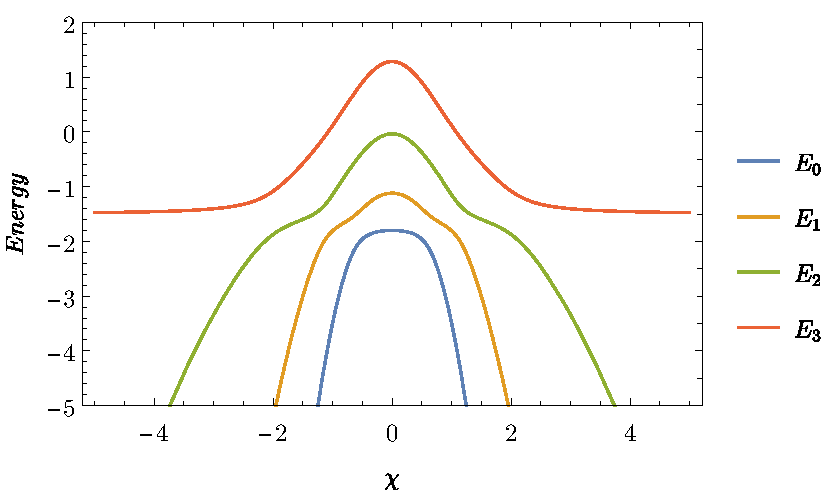
\includegraphics[scale=1.3]{../img/N=3_energiesl.pdf}
    \vspace{-3pt}\caption{Energy spectrum for $N=3$, section $\lambda=1$}
    \label{fig:N=3_energiesl}
\end{figure}
\begin{figure}[h]
    \centering
    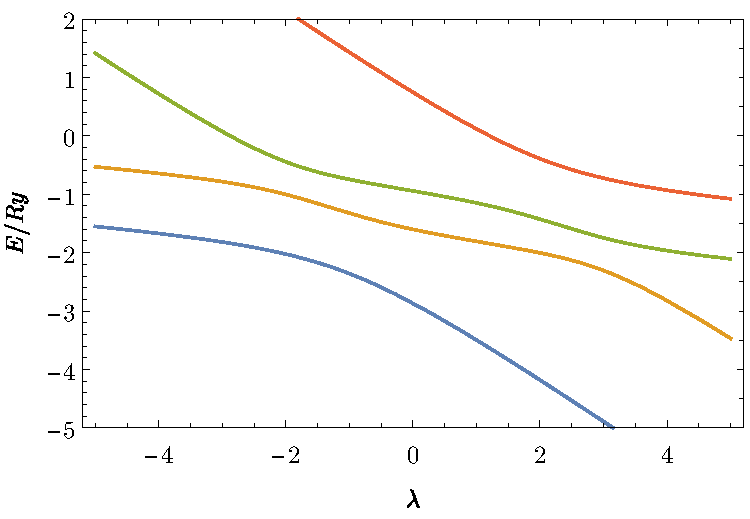
\includegraphics[scale=1.3]{../img/N=3_energiesc.pdf}
    \vspace{-3pt}\caption{Energy spectrum for $N=3$, section $\chi=1$.}
    \label{fig:N=3_energiesc}
\end{figure}

From Eq. \ref{eq:N=3_en0}, \ref{eq:N=3_en1} can be seen the possible existence of spectrum degeneracies between every two neighboring energy levels\footnote{If the functions $D,E,F,G$ were into real numbers, degeneracies would exist between every two neighboring energy levels. Because they are complex, the solution $E_i=E_j$ might not exist. From numerical results, degeneracies exist between every two neighboring energy levels.}. Degeneracy $\bluee{E_0}=\textcolor{orange}{E_1}$ holds for $D=E$, which for real values $\lambda,\;\chi$ has two solutions
\begin{equation}
    (\lambda_d,\pm \chi_d)=\left(-\frac{1}{2};\sqrt{\frac{3}{5}}\right).
\end{equation}
According to Theorem \ref{thm:n-2}, Hamiltonian driven by two real parameters can be degenerated only on 0-dimensional manifolds. This means that degeneracies are separated points in the parametric space.

If the energy spectrum is degenerate and the metric tensor diverges, see individual elements in Fig. \ref{fig:N=3_g}, its determinant also diverges, as shown in Fig. \ref{fig:N=3_gDivenrgence}, along with Christoffel symbols in Fig. \ref{fig:N=3_G}. The metric tensor determinant is positive definite; therefore, the manifold is Riemannian. Further on, it reflects the symmetry $\chi\leftrightarrow-\chi$, except for elements $g_{12}$, $\Gamma_{121}$, $\Gamma_{211}$, and $\Gamma_{222}$, which switch their sign.

Due to the metric tensor degeneracy, the space is not geodesically maximal. To see that the singularity is not only a \emph{coordinate one}\footnote{Coordinate singularity is present only in some coordinates. This is different from the so-called \emph{physical singularity}, which is present in every choice of the coordinate system.} the Ricci scalar can be calculated, see Fig. \ref{fig:N=3_Ricci}. Divergent Ricci scalar implies that singularity is physical. The diverging tendency for sections close to the point of degeneracy can be seen from sections in $\chi$-direction drawn in Fig. \ref{fig:N=3_Ricci_section}, which at coordinate $(\lambda_d;\chi_d)$ diverges. The coordinate independence of this singularity implies it is a\,\emph{physical singularity}. 


\begin{figure}[H]
    \centering
    \vspace{-30pt}\begin{tikzpicture}
        \node[] at (0,0) {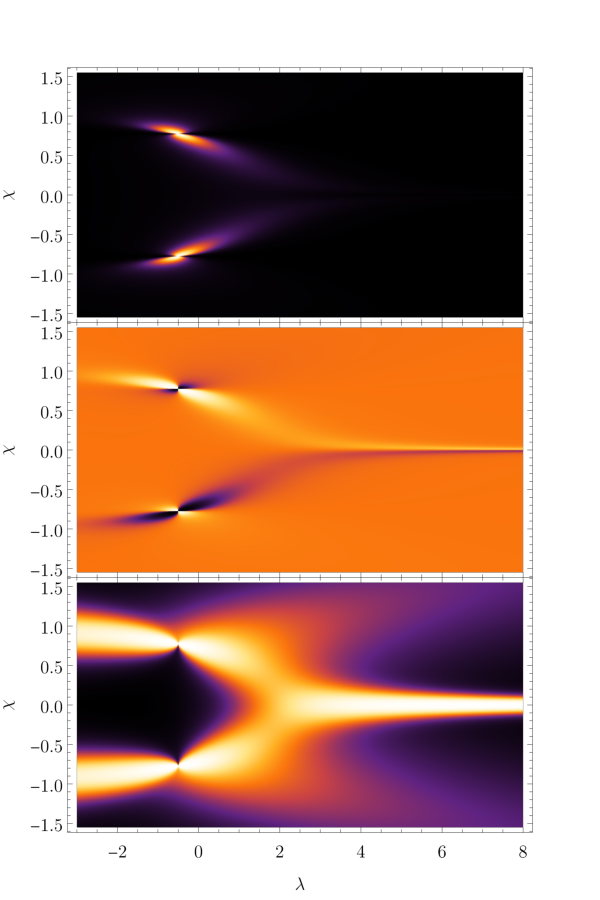
\includegraphics[scale=1.3]{../img/N=3_gComponents.pdf}};
        \node[] at (0,-11) {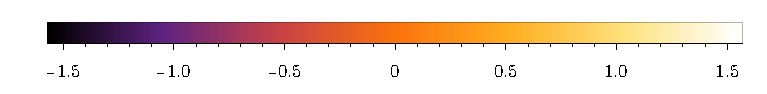
\includegraphics[scale=1.3]{../img/N=3_barA.pdf}};
        \node[] at (3.5,7.66) {\textcolor{white}{$\arctan(g_{11})$}};
        \node[] at (2.2,2.0) {\textcolor{white}{$\arctan(g_{12})=\arctan(g_{21})$}};
        \node[] at (3.5,-3.5) {\textcolor{white}{$\arctan(g_{22})$}};
    \end{tikzpicture}
\caption{Arctangent of the metric tensor elements for $N=3$ in the parametric space.}
    \label{fig:N=3_g}
\end{figure}

\begin{figure}[H]
    \centering
    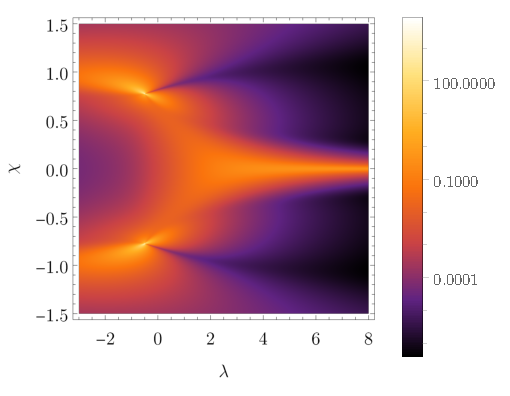
\includegraphics[scale=1.3]{../img/N=3_gDivergence.pdf}
    \caption{Ground state metric tensor determinant in a parametric space for $N=3$.}
    \label{fig:N=3_gDivenrgence}    
\end{figure}


\begin{figure}[H]
    \centering
    \vspace{-60pt}\begin{tikzpicture}
        \node[] at (0,0) {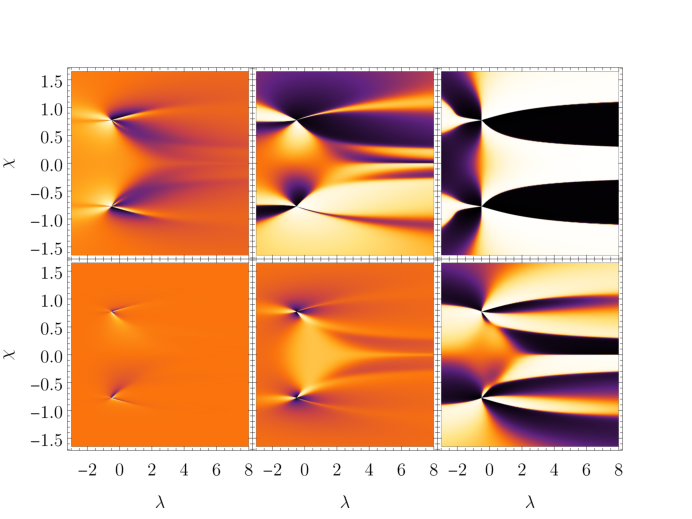
\includegraphics[scale=1.3]{../img/N=3_gammas.pdf}};
        \node[] at (-0.5,-6.5) {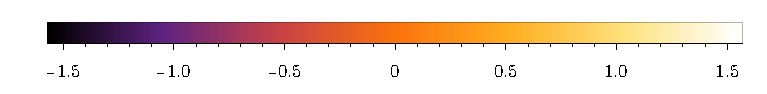
\includegraphics[scale=1.3]{../img/N=3_barA.pdf}};
        \node[] at (-3.4,0.5) {$\arctan(\Gamma_{111})$};
        \node[] at (0.7,0.5) {$\arctan(\Gamma_{121})$};
        \node[] at (4.75,0.5) {$\arctan(\Gamma_{122})$};
        \node[] at (-3.4,-0.5) {$\arctan(\Gamma_{211})$};
        \node[] at (0.7,-0.5) {$\arctan(\Gamma_{221})$};
        \node[] at (4.75,-0.5) {$\arctan(\Gamma_{222})$};
    \end{tikzpicture}
    \caption{Arctangent of the ground state Christoffel symbols for $N=3$.}
    \label{fig:N=3_G}
\end{figure}


\begin{figure}[H]
    \centering
    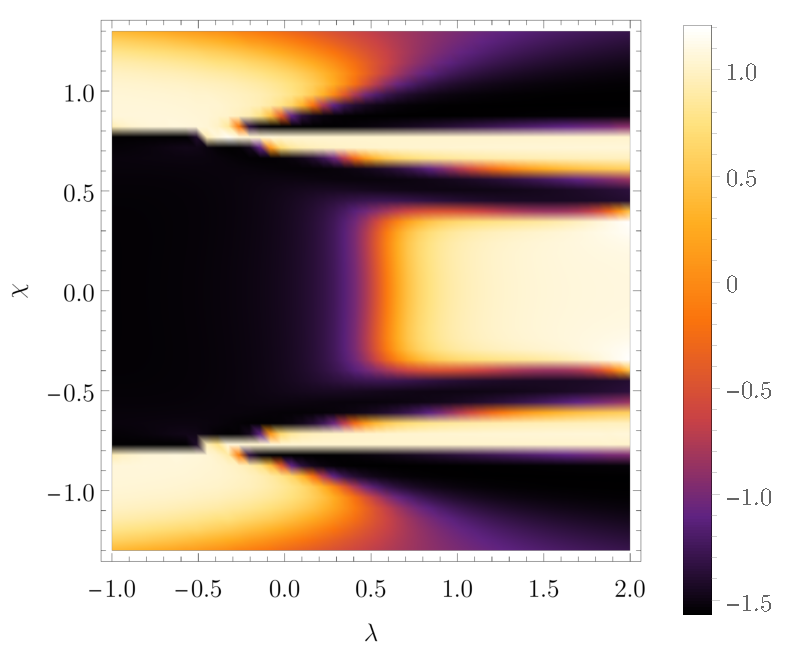
\includegraphics{../img/N=3_Ricci.pdf}
    \caption{Ricci curvature for the case $N=3$. The cutoff is set as $R_{min/max}=\pm1000$.}
    \label{fig:N=3_Ricci}
\end{figure}

% Coordinates of minima on lines with constant $\lambda$ in Ricci scalar can be seen in Fig. \ref{fig:N=3_RicMinimas} and will be important later on, because geodesics will be strongly repelled by parts of this line.
\begin{figure}[H]
    \centering
    \vspace{40pt}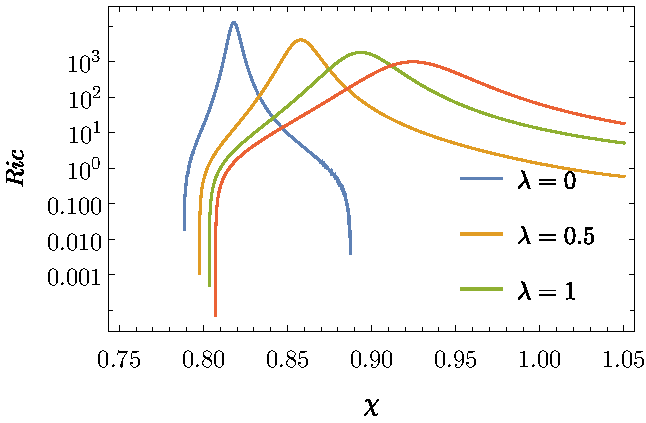
\includegraphics[scale=0.9]{../img/N=3_Ricci_section.pdf}
    \caption{Ricci curvature sections for three different $\lambda$. $N=3$.}
    \label{fig:N=3_Ricci_section}
\end{figure}
% \begin{figure}[h]
%     \centering
%     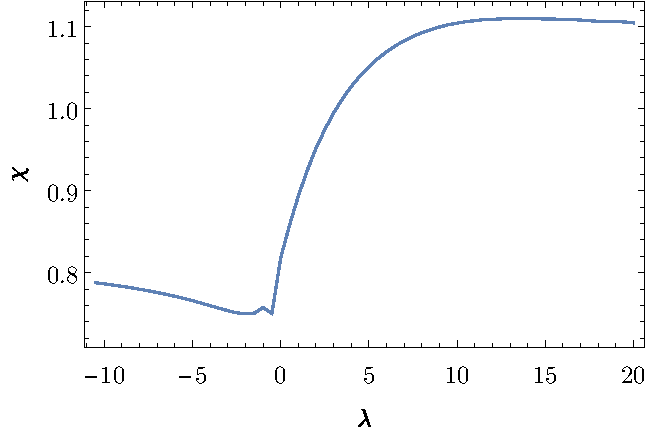
\includegraphics[scale=0.9]{../img/N=3_RicMinimas.pdf}
%     \caption{Minimas in Ricci curvature on the background of metric tensor determinant. Case $N=3$.}
%     \label{fig:N=3_RicMinimas}    
% \end{figure}

\newpage
\subsubsection{Geodesics}
The importance of geodesics was described in Chapter \ref{chap:groundStateManifoldDriving}. In addition, they give a tool for observing some system characteristics, such as singularities, or curvature in general. \emph{Initial valued Geodesics} are solutions to
$$(\lambda(0);\chi(0))\eqqcolon (\lambda_i;\chi_i)$$
$$\left(\der{\lambda(t)}{t};\der{\chi(t)}{t}\right)\Bigg|_{t=0} \eqqcolon (\lambda'_i;\chi'_i),$$
where zero was set as an initial time.

One might also choose the \emph{boundary valued geodesics} with fixed initial and final position, $(\lambda(0);\chi(0))$ and $(\lambda(T);\chi(T))$ respective. Because the shape of geodesics in parametric space does not depend on the initial derivative, it does not depend on the speed of driving in the parametric space. Initial valued geodesics are therefore more advantageous to calculate because they have only three free parameters — the initial coordinates $(\lambda_i;\chi_i)$ and the ratio $\lambda'_i/\chi'_i$. Another reason is purely numeric, which is that the boundary-valued geodesics are calculated by numerous evolutions of the initial valued geodesics. Usually the software evolves many initial valued geodesics and checks if the final boundary condition is satisfied. If not, the initial parameters are tweaked in response until it fits the boundary condition. Calculating the boundary valued geodesics is generally much slower. In this case, the calculation time was $10$ to $100$ times longer.

Results for geodesics starting at $(\lambda_i;\chi_i)=(0;0)$, $
(\lambda',\chi')=(\cos\theta;\sin\theta)$ can be seen in Fig. \ref{fig:N=3_geodesics}. Other values $\theta$ result in a close approach of the geodesics to the singularity, making the calculation numerically unstable. The fact that geodesics lean toward singularities is well known from the theory of General Relativity (GR). The main difference here is that our "test particle" seems to be partially repulsed by the singularity. The analogy with GR then fails because of the nonexistence of negative mass and gravitational dipoles. The better analogy is electromagnetism, which has a downside in the fact that geometrical formalism is not used so much in this theory. A comparison of these two intuitive examples can be seen in Fig. \ref{fig:geodesicsinGR}. The geodesic behavior is caused not only by the singularity but also by a large Ricci curvature leaning to the right from it. This means the distance across this \emph{\blueee{unreachable gap}}, marked by \blueee{blue line} in Fig. \ref{fig:N=3_geodesics}, is also large. The geodesics then have a strong tendency to avoid its crossing. The presence of singularities means that our ground state manifold is geodesically incomplete, and according to Theorem \ref{thm:hopf-Rinow_modified}, there exist some geodesically unreachable coordinates. From this goes the term \emph{\blueee{unreachable gap}}.

The fact that geodesics lean toward singularities and parts of parametric space with small energy level difference $\Delta E$ implies that for general fidelity driving, the geodesics cannot be advantageous in the case of fidelity. The excitation probability increases with smaller $\Delta E$ leading to a fidelity decrease for such drivings.


\begin{figure}[H]
    \centering
    % 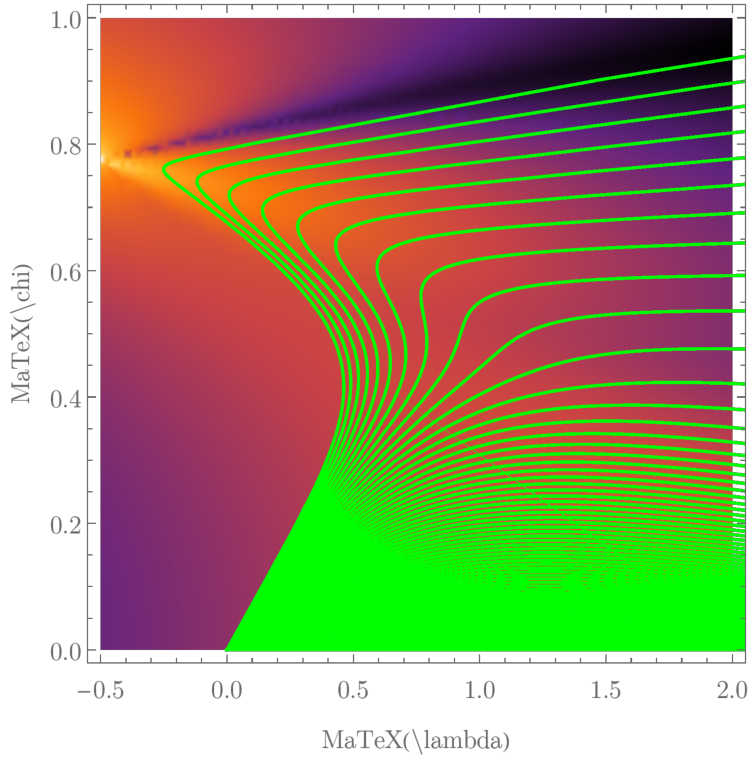
\includegraphics{../img/N=3_geodesics.pdf}
    \begin{tikzpicture}
        \node[anchor=south west,inner sep=0] at (0,0) {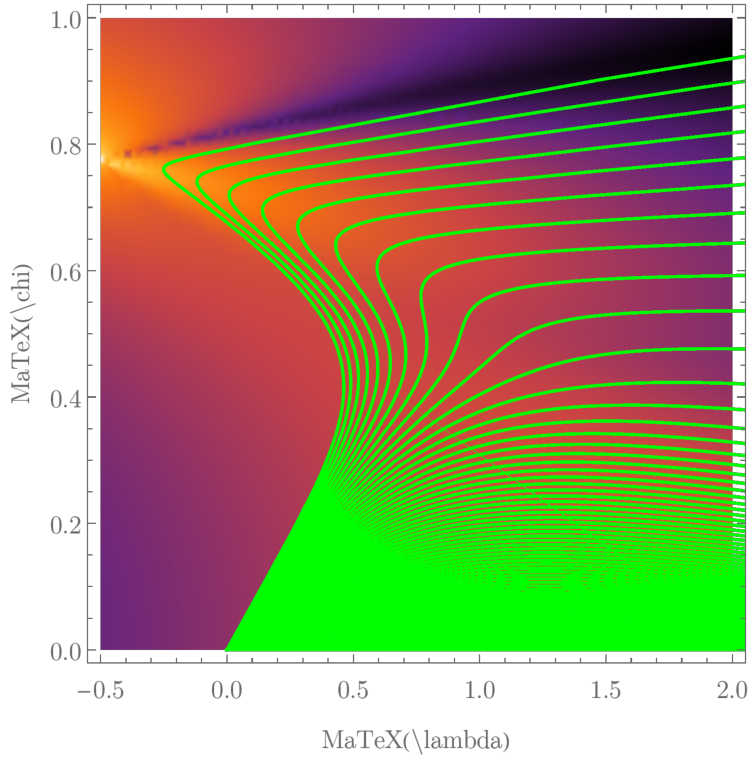
\includegraphics{../img/N=3_geodesics.pdf}};
        \draw[blueee,ultra thick] (4.5,9.56) -- (10.67,10.5);
        \draw[blueee,ultra thick] (4.5,2.71) -- (10.67,1.8);
    \end{tikzpicture}
    \vspace{-10pt}\caption{\green{Geodesics} for $N=3$ starting from $(\lambda_i;\chi_i)=(0;0)$ with $(\lambda'_i;\chi'_i)=(\cos\theta;\sin\theta)$, parametrized by angle $\theta\in [-0.63;0.63]$, $\theta\in [\pi-0.225;\pi+0.225]$, with step $\Delta\theta=0.01$. \blueee{Blue} line marks the \blueee{unreachable gap}, where the Ricci curvature is big.}
    \label{fig:N=3_geodesics}    
\end{figure}



\begin{figure}[H]
    \centering
    \vspace{30pt}\begin{tikzpicture}
        \node[] at (0,0) {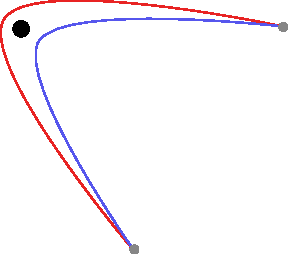
\includegraphics[width=0.3\textwidth]{../img/comparingGeodesics.pdf}};
        \node[] at (-3.2,1.53) {singularity};
        \node[] at (3.0,1.5) {\gray{$(\lambda_i;\chi_i)$}};
        \node[] at (0.8,-1.9) {\gray{$(\lambda_f;\chi_f)$}};        
    \end{tikzpicture}
    \caption{Comparing the \gray{boundary} valued geodesics for \blue{repulsing (inner line)} and \red{attracting (outer line)} metric tensor divergence in the spherically symmetrical space. }
    \label{fig:geodesicsinGR}
\end{figure}



% \begin{figure}[h]
%     \centering
%     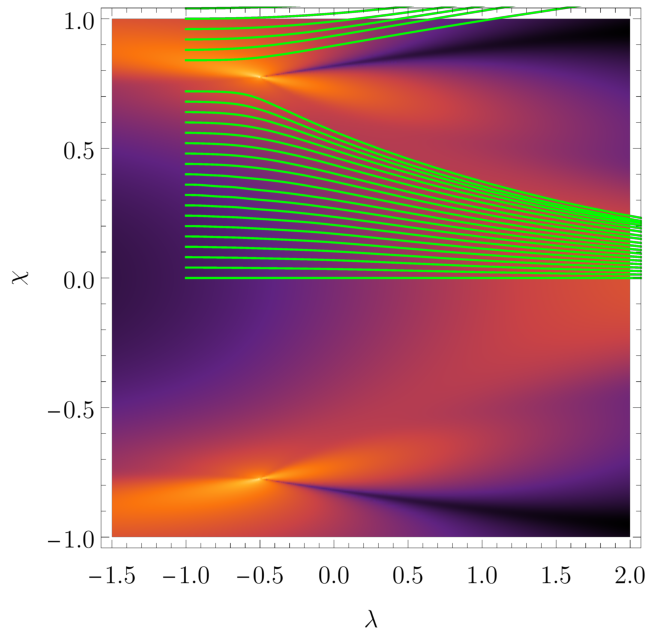
\includegraphics{../img/N=3_geodesics_lambdaIn=-1.pdf}
%     \caption{Geodesics starting from $(\lambda_i;\chi_i)=(-1;\chi_i)$, $(\lambda',\chi')=(1;0)$, for $\chi_i\in(0;1)$ with step $0.05$. Numerically unstable geodesics were skipped. Case $N=3$.}
%     \label{fig:N=3_geodesics_lambdaIn=-1}    
% \end{figure}


\newpage
\subsection{5-dimensional Hamiltonian}
Another special case is $N=5$. The ground state manifold can be understood from the metric tensor determinant, see Fig. \ref{fig:N=5_det3D}. Here we see the spectrum degeneracy causes high positive values of metric tensor determinant and the \blueee{unreachable gap} is characterized by small determinant values. 

Between every two neighboring energy levels, there are many degeneracies, as can be seen in Fig. \ref{fig:singularitiesBetweenEnergiesN=5}. $E_0=E_1$ degeneracy lies approximately on the line called the \emph{separatrix} (see Chap. \ref{chap:infiniteDimensionLimit}) and other singularities are distributed around. The $\chi\leftrightarrow-\chi$ symmetry holds for all of them.



Geodesics for the case $N=5$ starting at $(\lambda;\chi)=(0;0)$ have similar characteristics to the case $N=3$. However, the behavior around the singularity is not the only interesting thing happening. Another phenomenon arises for the initial coordinates in the higher curvature around $(1;0)$. As can be seen in Fig. \ref{fig:geod10}, the geodesics tend to deflect themselves from the area with high curvature around the axis $\chi=0$. This effect is present even for the initial coordinate $(0;0)$, but it is not so apparent. Small irregularity can be seen in Fig. \ref{fig:N=3_geodesics} around point $(0.5;0.1)$ and means that the geodesic equation might have at least two solutions as candidates for the globally shortest path between two points.\footnote{One might recall the effect of gravitational lensing here. In the presence of any mass in spacetime, there exist more possible light paths (solutions to the geodesic equation) between two points, differing by the initial condition.} 

\begin{figure}[H]
    \centering
    \vspace{20pt}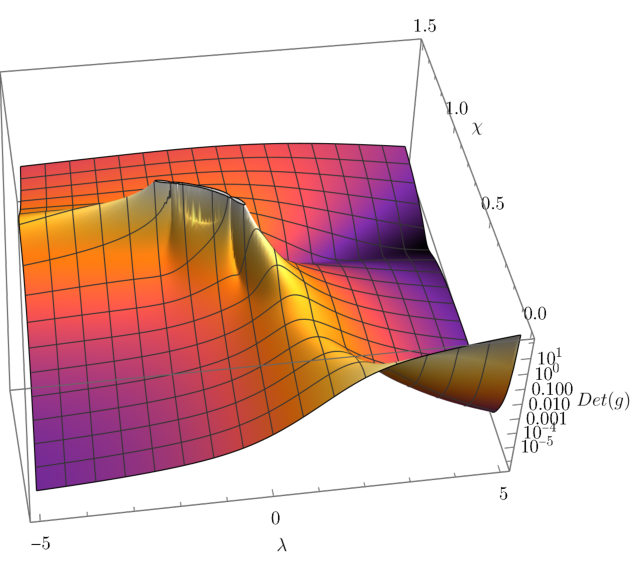
\includegraphics[scale=1.3]{../img/N=5_det3D.pdf}
    \caption{Metric tensor determinant for the case $N=5$.}
    \label{fig:N=5_det3D}    
\end{figure}

\begin{figure}[H]
    \centering
    \begin{tikzpicture}
        \node[] at (0,0) {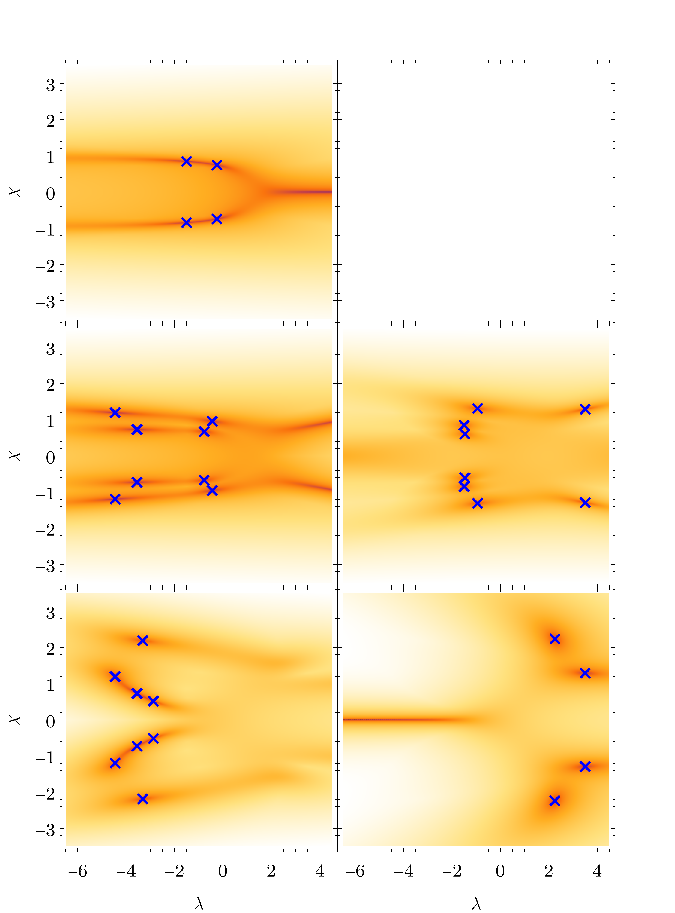
\includegraphics[scale=1.3]{../img/singularitiesBetweenEnergiesN=5.pdf}};
        \node[] at (-1.1,8.2) {$E_1-E_0$};
        \node[] at (-1.1,2.2) {$E_2-E_1$};
        \node[] at (5,2.2) {$E_3-E_2$};
        \node[] at (-1.1,-3.5) {$E_4-E_3$};
        \node[] at (5,-3.4) {$E_5-E_4$};
    \end{tikzpicture}
    \caption{Energy differences between neighboring energy levels for $N=5$. Spectra degeneracies are marked with \blue{blue cross}.
    % First row: $E_1-E_0$, second row from left: $E_2-E_1$, $E_3-E_2$, third row from left: $E_4-E_3$, $E_5-E_4$. 
    }
    \label{fig:singularitiesBetweenEnergiesN=5}   
\end{figure}



\begin{figure}[H]
    \centering
    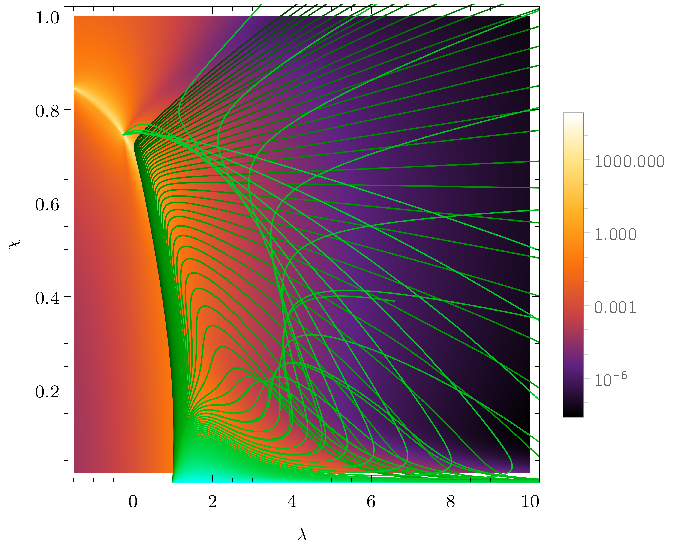
\includegraphics[scale=1.3]{../img/N=5_geods00.pdf}
    \caption{Geodesics for the case $N=5$, starting at $(1;0)$. The numerics for geodesics passing close to the singularity can be observed to break down — their evaluation stopped.}
    \label{fig:geod10}    
\end{figure}

% \begin{figure}[h]
%     \centering
%     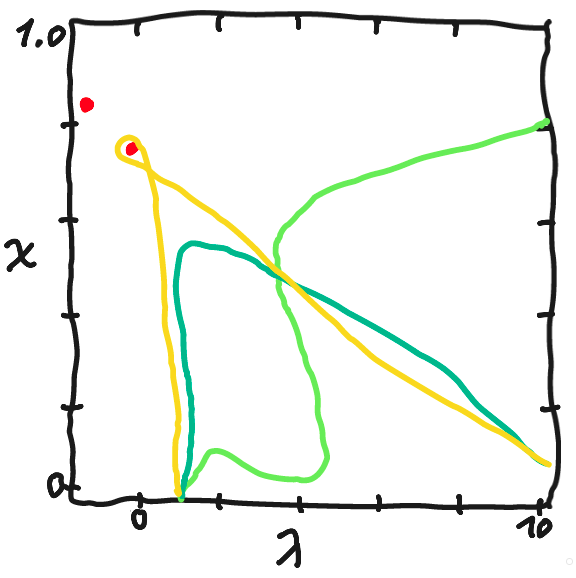
\includegraphics[scale=0.35]{../img/geodesicSolutionsDrawing.png}
%     \caption{Three possible solutions between points $(1;0)$ and $(4;0.5)$. The length of the yellow one is surely longer than other two, but the difference between green vs. blue solution is not clear on the first sight.}
%     \label{fig:geodesicsBetweenPoints}    
% \end{figure}






\subsection{Infinite dimension limit}
\label{chap:infiniteDimensionLimit}
The limit $N\rightarrow \infty$ can be taken from Hamiltonian in Eq. \ref{eq:firstOrderTransitionHamiltonian} using Holstein-Primakoff mapping \citet{holstein} for bosonic operators
\begin{equation}
    \mathcal{H}\coloneqq\lim_{j\rightarrow\infty}\frac{\HH}{2j},
\end{equation}
resulting in classical Hamiltonian
\begin{equation}
    \begin{split}
        \mathcal{H}(x,p)=&-\frac{1}{2}+\frac{1-\lambda}{2}x^2+\frac{\lambda-\chi^2}{4}x^4-\frac{\chi x^3}{2}\sqrt{2-x^2-p^2}-\frac{\chi^2}{4}p^4\\
        &+\frac{p^2}{4}\left[2+(\lambda-2\chi^2)x^2-2\chi x\sqrt{2-x^2-p^2}\right].
    \end{split}
    \label{eq:HamiltonianClassicalLimit}
\end{equation}
For more, see \citet{felipe}.

The minima of function $\H(x,p)$ form a line, called the \emph{separatrix}. In this case it can be expressed as
\begin{equation}
    \chi^2=\frac{\lambda-1}{\lambda-2}.
    \label{eq:separatrix}
\end{equation}
The separatrix represents phase transition in the limit $N\rightarrow \infty$. In the case of the LMG model, the transition is of first-order everywhere, except in $(\lambda;\chi)=(1;0)$, 
\begin{figure}[h]
    \centering
    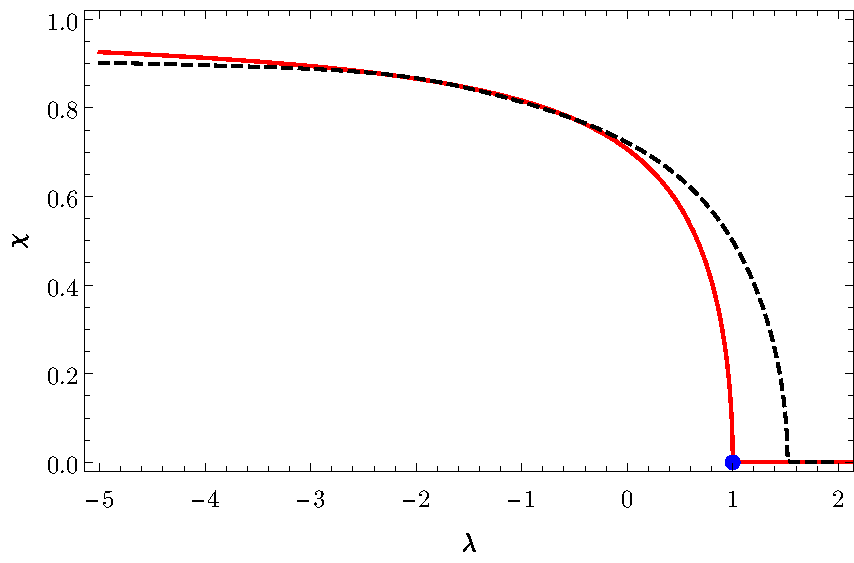
\includegraphics[scale=1.2]{../img/infiniteN_transitionCompare.pdf}
    \caption{\red{First order phase transition, the separatrix (red line)}, \blue{second order transition (blue point)} compared to the \emph{minimal line in N=3 case} (black, dashed).}
    \label{fig:transitionCompare}    
\end{figure}
where it has order two. The separatrix is shown in Fig. \ref{fig:transitionCompare} compared to the minimum of $E_1-E_0$ line, so-called the \emph{minimal line}. With increasing $N$, it converges to the separatrix. The driving over the first-order transition is generally more advantageous than when the transition is of the second order. The reason is in the $E_1-E_0$ dependence on system dimension $N$. For details, see \citet{shuetzhold}.











\section{General spectrum behavior}
In higher dimensions $N$ we see the same characteristic behavior in the energy spectrum sections, see the example in Fig. \ref{fig:N=10_energiesl}, \ref{fig:N=10_energies2} for $N=10$ case. It is not yet clear if there is a degeneracy between every two neighboring energy levels. From numerical observation on $N<10$ goes that there are $N-2$ crossings for $N$ odd and $N-3$ for $N$ even. Here the analytical proof needs to be found.


Special attention is given to the spectrum degeneracies between zeroth and first energy level because these influence the metric tensor and ground-state manifold geodesics the most. Their exact calculation is numerically expensive, and only the first few cases, namely, $N\in\{3,4,5,6,7\}$, were calculated, see Tab. \ref{tab:singularities}. 
\begin{table}[h]
    \centering
    \vspace{-3pt}\begin{tabular}{c||c|c|c}
     N&$(\lambda_l;\pm\chi_l)$&$(\lambda_2;\pm\chi_2)$&$(\lambda_r;\pm\chi_r)$        \\ \hline\hline
     3&$(-\frac{1}{2};\sqrt{\frac{3}{5}}) $&                                       &                                         \\
     4&$(-3          ;\sqrt{\frac{4}{5}}) $&                                       & $(-\frac{1}{3};\sqrt{\frac{4}{7}})$     \\
     5&$(-\frac{3}{2};\sqrt{\frac{5}{7}}) $&                                       & $(-\frac{1}{4};\sqrt{\frac{5}{9}})$     \\
     6&$(-5          ;\sqrt{\frac{6}{7}}) $&$(-1          ;\sqrt{\frac{2}{3}}) $   & $(-\frac{1}{5};\sqrt{\frac{6}{11}})$     \\
     7&$(-\frac{5}{2};\sqrt{\frac{7}{9}}) $&$(-\frac{3}{4};\sqrt{\frac{7}{11}}) $  & $(-\frac{1}{6};\sqrt{\frac{7}{13}})$ 
    \end{tabular}
    \caption{Singularities between the zeroth and first energy levels for dimensions 3--7. Subscript $l(r)$ means the most \emph{left(right)-wise} positioned coordinates in the $(\lambda,\chi)$-plot.}
    \label{tab:singularities}
    \end{table} 

From the singularity behavior in low dimensions, one might see the pattern for $(\lambda_l,\chi_l)$ and $(\lambda_r,\chi_r)$, i.e., those with minimal, resp maximal $\lambda$ coordinate

\begin{equation}
    (\lambda_l ;\pm\chi_l)= \begin{cases}
        \left(1-\frac{N}{2};\sqrt{\frac{N}{N+2}}\right) & , N\geq 3,N\text{ is odd}\\
        \left(1-N;\sqrt{\frac{N}{N+1}}\right) & , N\geq 3,N\text{ is even}
    \end{cases}
    \label{eq:singularityCoordinateFormulaLeft}
\end{equation}
\begin{equation}
    (\lambda_r ;\pm\chi_r)= 
        \left(\frac{1}{1-N};\sqrt{\frac{N}{2N-1}}\right)\quad , N\geq 3.
        \label{eq:singularityCoordinateFormulaRight}
\end{equation}
These were numerically proven to be singularities for cases up to $N=1000$. 

The singularities in dimensions 3 to 10 are shown in Fig. \ref{fig:singularities3to10} along with the metric tensors determinant for corresponding state manifolds.
In addition, the degeneracies between zeroth and first energy levels belong to the minimal line, which is close to the separatrix described by Eq. \ref{eq:separatrix}. Due to this, the position of singularities is constrained to the \emph{second order phase transition line} between points $(\lambda_l,\pm\chi_l)$ and $(\lambda_r,\pm\chi_r)$. In the limit $N\rightarrow\infty$ they converge to
\begin{align*}
    \lim_{N\rightarrow \infty}(\lambda_l ;\pm\chi_l)&= \left(-\infty,1\right)\\
    \lim_{N\rightarrow \infty}(\lambda_r ;\pm\chi_r)&= \left(0,\frac{1}{\sqrt{2}}\right).
\end{align*}

It is still unclear if in the limit $N\rightarrow \infty$ the singularities cover the whole part $\lambda<0$ of the separatrix.



\begin{figure}[h]
    \centering
    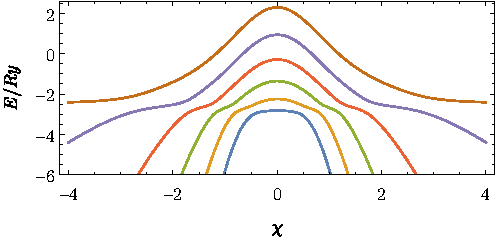
\includegraphics[scale=1.4]{../img/N=10_energiesl.pdf}
    \vspace{-1pt}\caption{The energy spectrum as a function of $\chi$. $\lambda=1$ and $N=10$.}
    \label{fig:N=10_energiesl}    
\end{figure}
\begin{figure}[h]
    \centering
    \vspace{-18pt}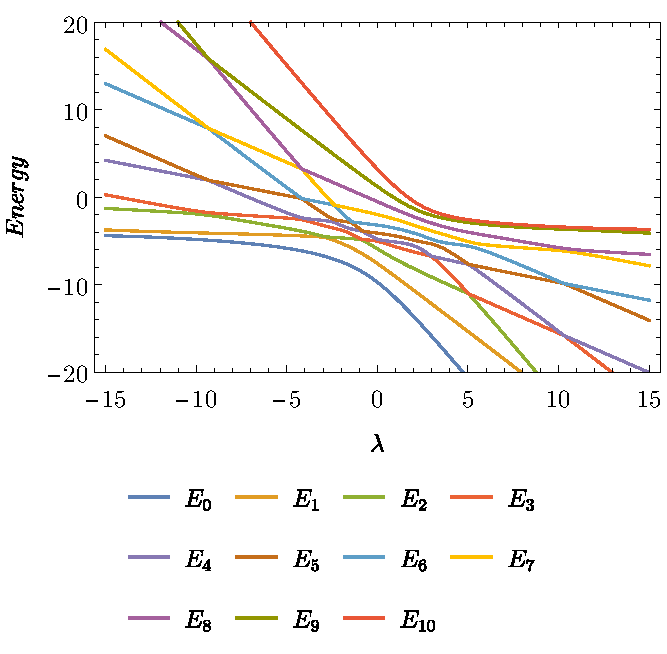
\includegraphics[scale=1.4]{../img/N=10_energies2.pdf}
    \vspace{-1pt}\caption{The energy spectrum as a function of $\lambda$. $\chi=1$ and $N=10$.}
    \label{fig:N=10_energies2}    
\end{figure}


\begin{figure}[h]
    \centering
    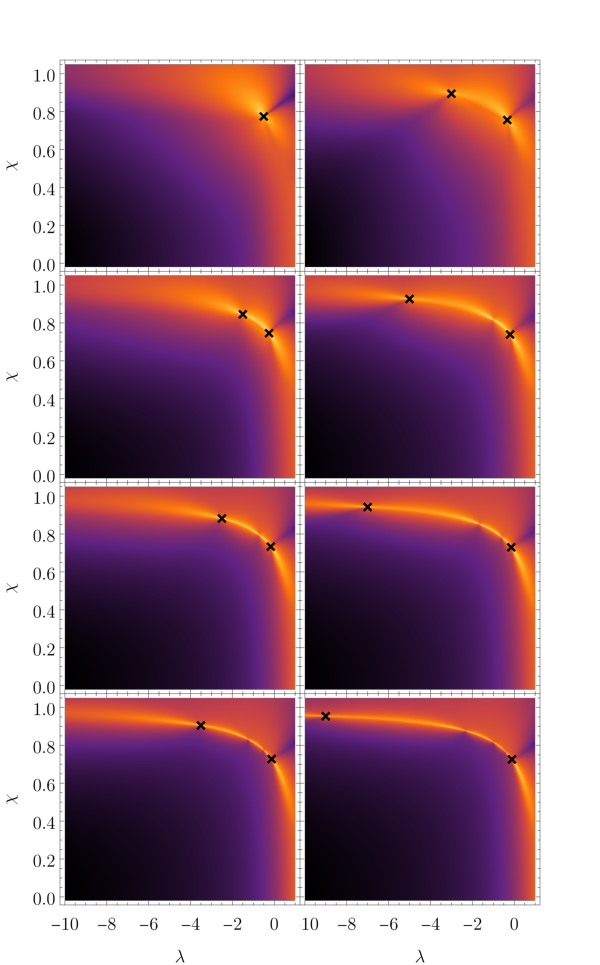
\includegraphics[scale=1.3]{../img/singularitiesPlots.pdf}
    \caption{Spectrum degeneracies between $E_0$ and $E_1$. Hamiltonian dimensions are 3,5,7,9 in the first column and 4,6,8,10 in the second column. Black crosses mark most left-wise and right-wise singularity and the background corresponds to the metric tensor determinant. Other singularities are also well visible in the determinant as defects on the \emph{high determinant value line}.}
    \label{fig:singularities3to10}    
\end{figure}









% \section{Higher state manifolds}



% \begin{figure}[h]
%     \centering
%     \includegraphics[scale=1.2]{../img/N=5_metricDeterminants.pdf}
%     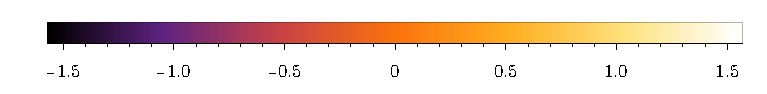
\includegraphics[scale=1.2]{../img/N=3_barA.pdf}
%     \caption{Arctangens of the metric tensor for higher state manifolds. By  rows: $M_0$, $M_1$; $M_2$, $M_3$; $M_4$, $M_5$.}
%     \label{fig:higherStateManifolds}    
% \end{figure}


% \begin{figure}[h]
%     \centering
%     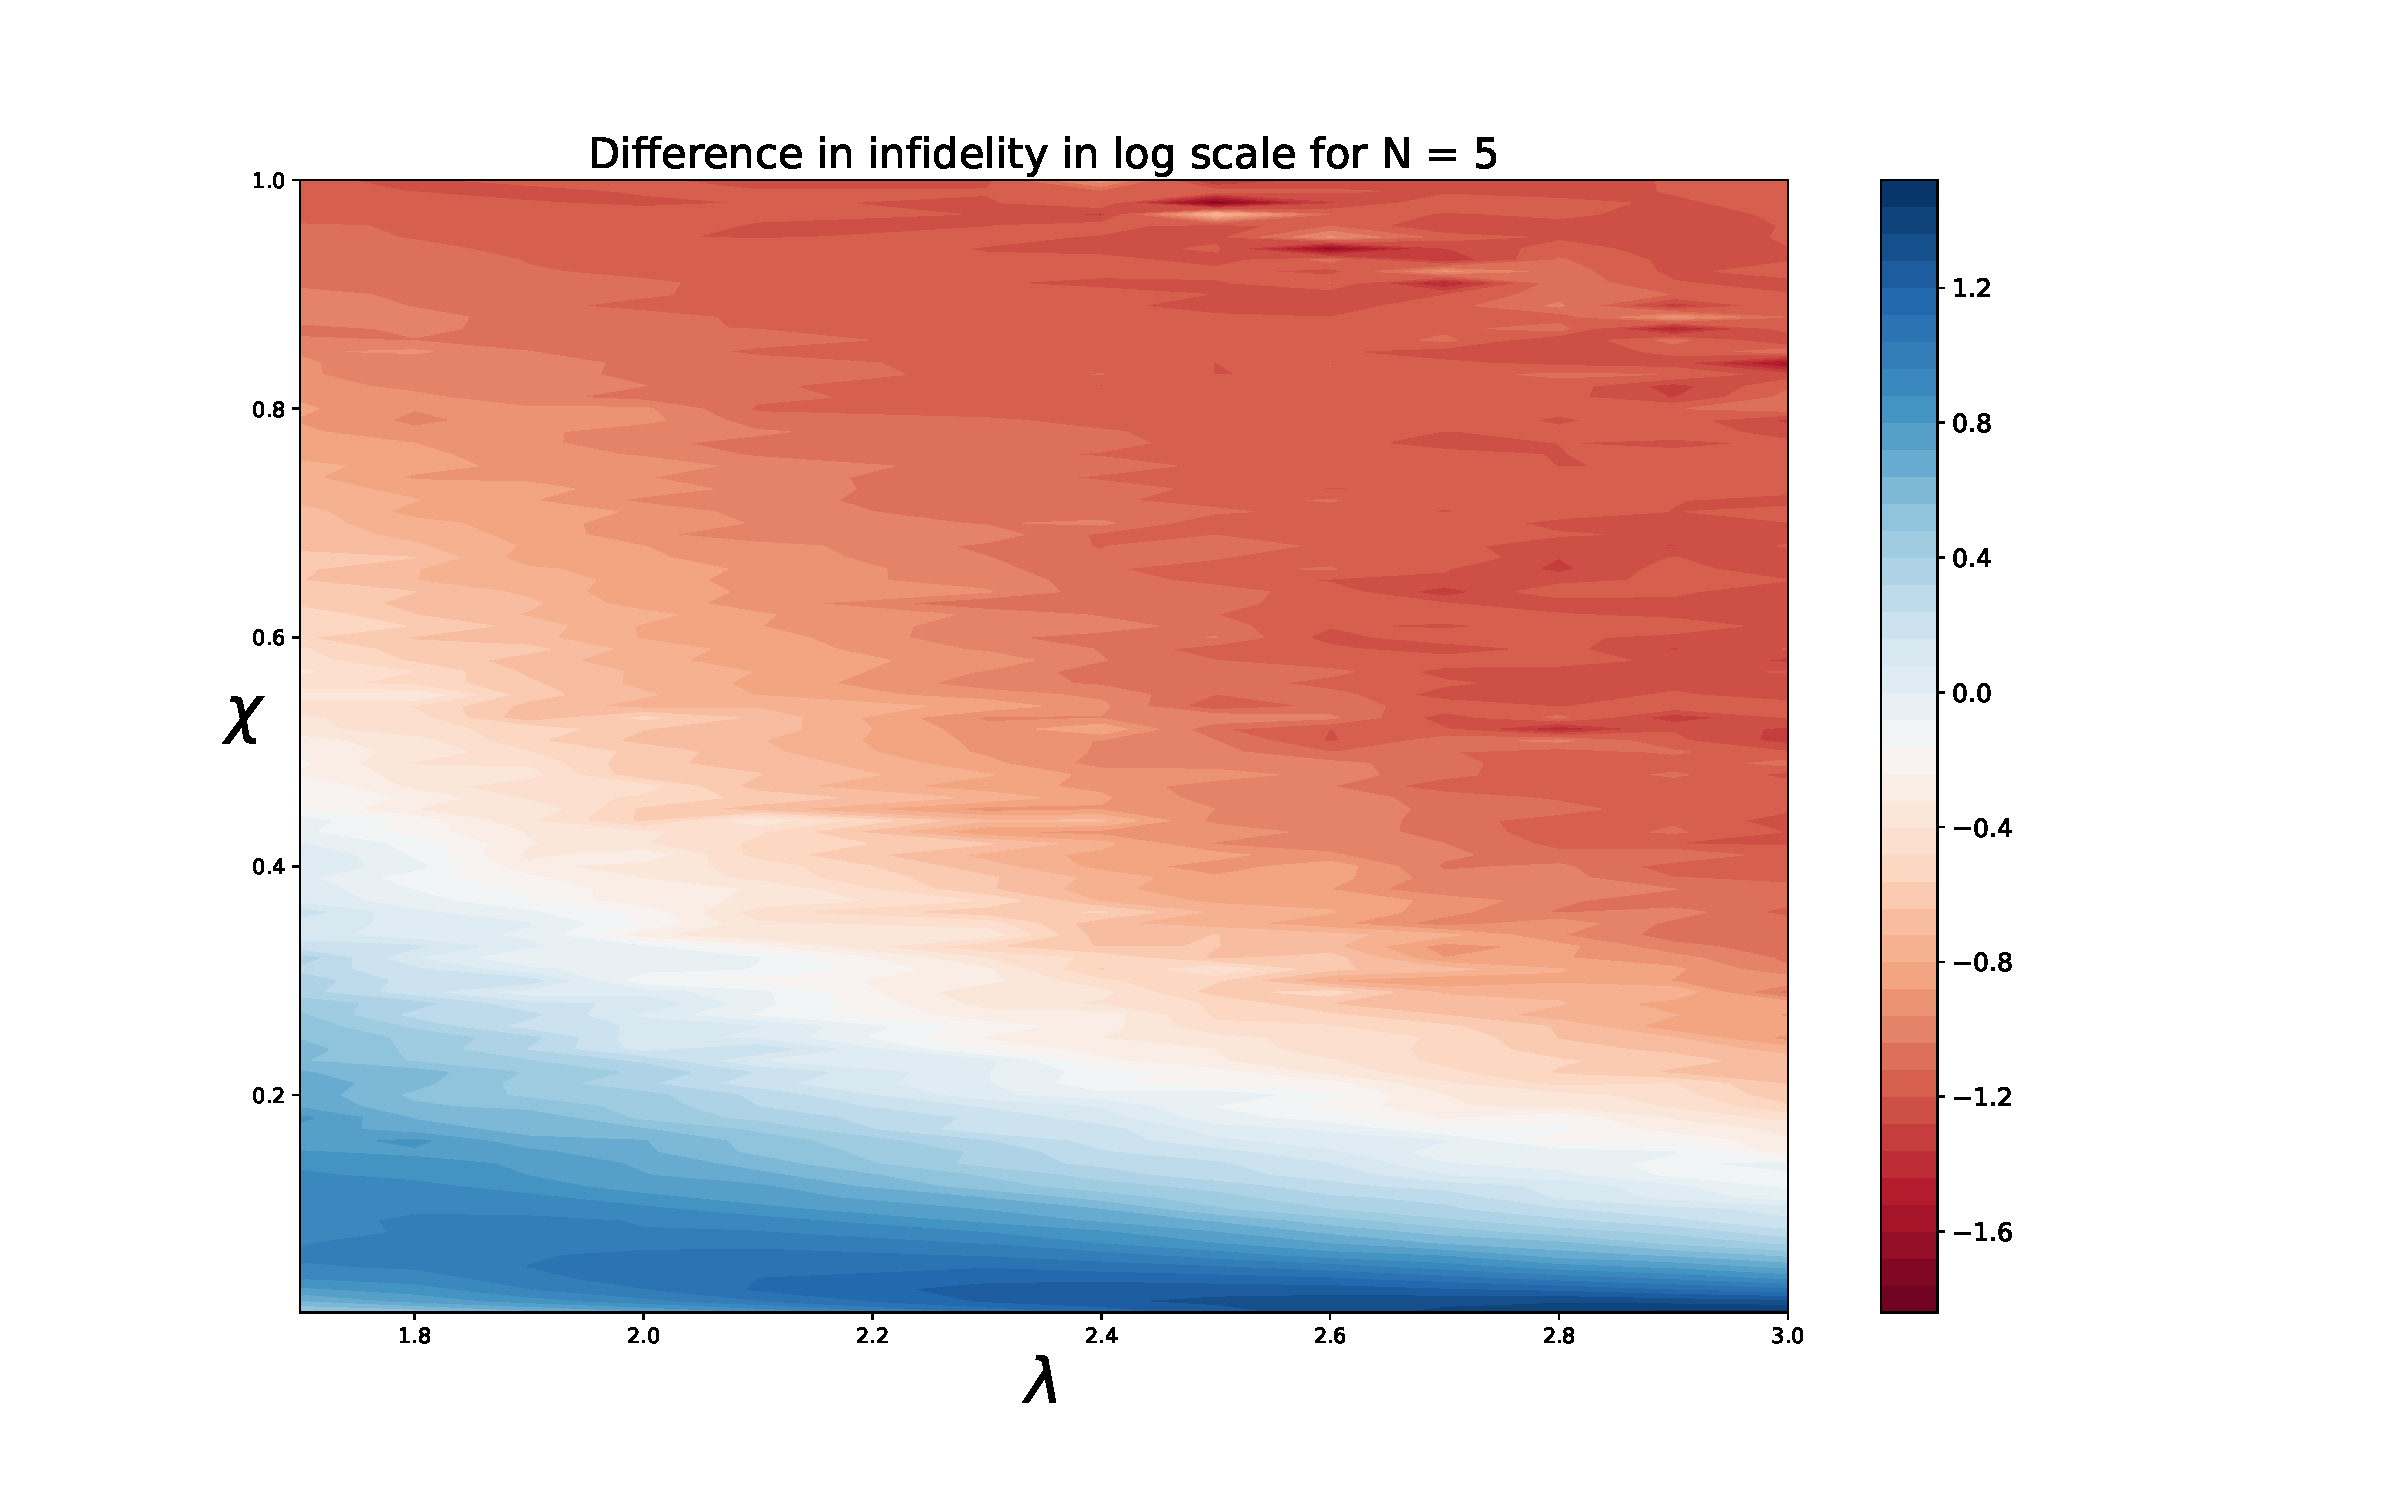
\includegraphics[width=1\textwidth]{../img/fidelity_lineVSgeodesic.pdf}
%     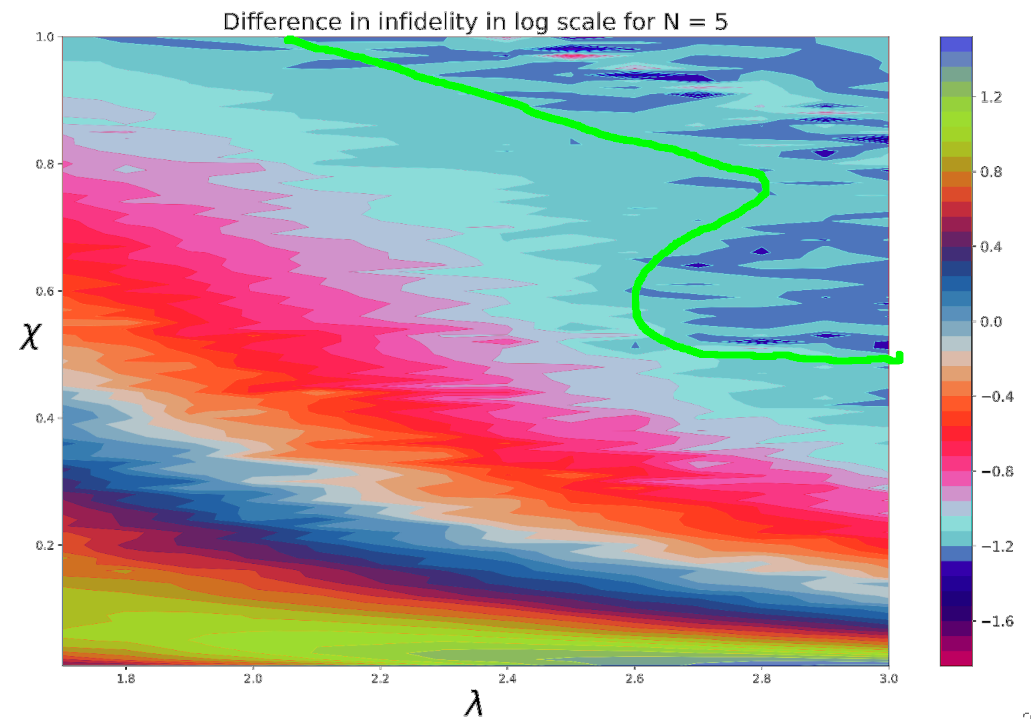
\includegraphics[width=0.8\textwidth]{../img/fidelity_geodesicVSline_fuckedupcolors.png}
%     \caption{\textcolor{gray}{Infidelity difference between line and geodesic, above picture is original from Felipe, bottom one is edited in GIMP to see the difference more clearly.}}
%     \label{fig:higherStateManifolds}    
% \end{figure}
